% Created 2019-01-21 Mon 22:09
% Intended LaTeX compiler: pdflatex
\documentclass[bigger]{beamer}
\usepackage[utf8]{inputenc}
\usepackage[T1]{fontenc}
\usepackage{graphicx}
\usepackage{grffile}
\usepackage{longtable}
\usepackage{wrapfig}
\usepackage{rotating}
\usepackage[normalem]{ulem}
\usepackage{amsmath}
\usepackage{textcomp}
\usepackage{amssymb}
\usepackage{capt-of}
\usepackage{hyperref}
\usepackage{fontspec}
\usepackage{natbib}
\usepackage{tikz}
\usepackage{bm}
\usepackage{minted}
\newcommand{\exV}[1]{\mathbb{E} \left [ #1 \right ]}
\usetheme{Montpellier}
\author{Timothy Schwieg}
\date{\today}
\title{The benefits of Randomization Mechanisms in Counter-Strike: Global Offensive}
\hypersetup{
 pdfauthor={Timothy Schwieg},
 pdftitle={The benefits of Randomization Mechanisms in Counter-Strike: Global Offensive},
 pdfkeywords={},
 pdfsubject={},
 pdfcreator={Emacs 26.1.50 (Org mode 9.1.9)}, 
 pdflang={English}}
\begin{document}

\maketitle

\section{Thesis}
\label{sec:org92d0972}
\begin{frame}[label={sec:org6792b65}]{Topic}
\begin{itemize}
\item Many video games have chosen to sell cosmetic alterations to their
games using randomization mechanisms called ``loot boxes''
\item Economic Literature tells us that there is no benefit to
randomization for risk-neutral consumers, so the benefit must come
from risk-loving consumers.
\item How much more revenue-generating is this compared to traditional
selling mechanisms?
\end{itemize}
\end{frame}

\section{Counter-Strike}
\label{sec:org0597353}
\begin{frame}[label={sec:org27a13c0}]{What is Counter Strike?}
\begin{itemize}
\item Popular First-Person Shooter video game first created in 1999,
current version has existed since 2012
\item Weapon Skins are items that change how your weapon looks within the game
\item Skins can be opened from boxes for \(\$2.50\) or bought and sold at
a secondary market
\item The contents are each box are public, as are the probabilities of
obtaining each of the contents.
\item The boxes or their contents are able to be sold at a
secondary market where Valve then takes 15\% as a tax.
\end{itemize}
\end{frame}

\begin{frame}[label={sec:org5261429}]{Why do we care?}
\begin{itemize}
\item We are interested in discovering what drives this market to feature
randomization mechanisms.
\item Are consumers inherently more risk-loving when they play video
games?
\item Is this driven by consumers over-weighting tiny probabilities as
cumulative prospect theory suggests?
\item Are consumers weighing benefits and losses differently?
\item What is the magnitude of these gains from randomization?
\end{itemize}
\end{frame}

\begin{frame}[label={sec:orgb7280d7}]{What do the weapon skins look like?}
\begin{figure}[H]
  \centering
  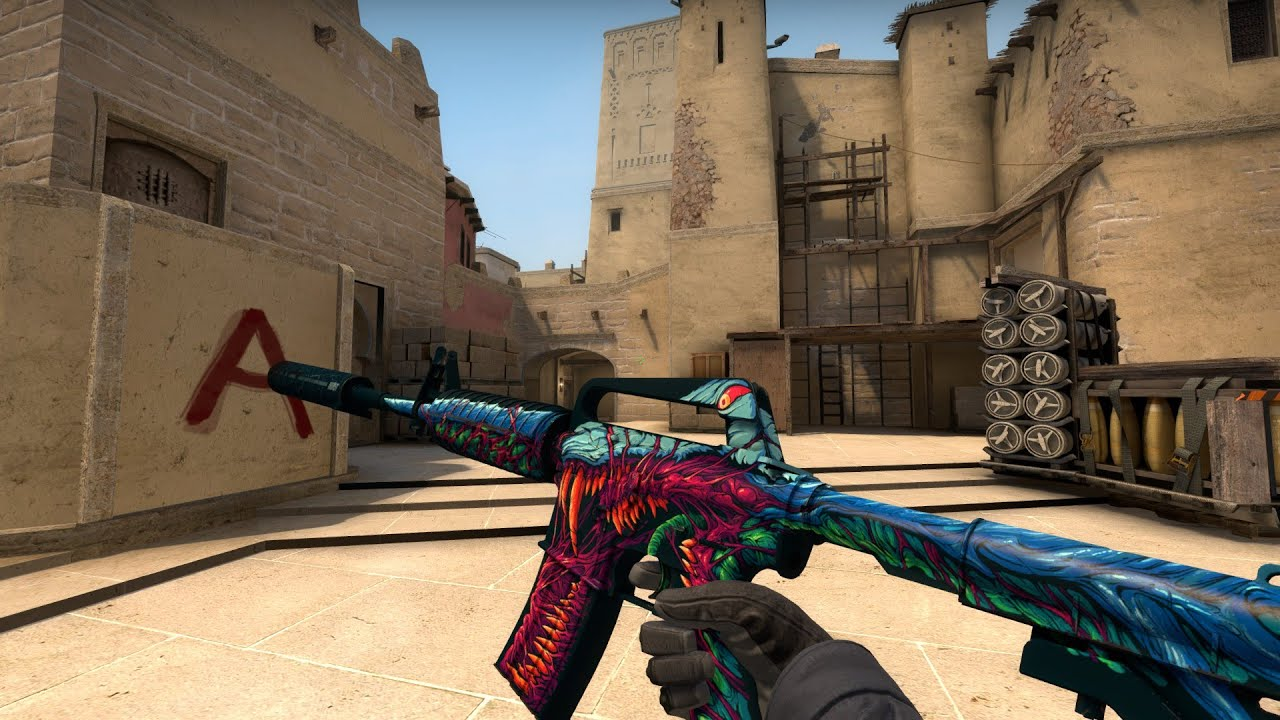
\includegraphics[width=8cm]{hyperBeast.jpg}
\end{figure}
\end{frame}


\section{Data}
\label{sec:org637e455}
\begin{frame}[label={sec:orge2612e9}]{The Data}
\begin{itemize}
\item Contains complete market history for all items sold in the Steam
Community Market for \emph{Counter-Strike: Global Offensive}
\item Market history is specific to the hour for the last 30 days,
specific to the day for the remaining time the item has existed.
\item Contains all active buy and sell orders for each of these items as
of June 7\(^{\text{th}}\) 2018.
\item Note that this not the only way to obtain the item, as it can also
be obtained by opening the box.
\end{itemize}
\end{frame}



\section{Model}
\label{sec:orgdba4b2f}
\begin{frame}[label={sec:org21a6ba3}]{Roadmap}
\begin{itemize}
\item Want to estimate the demand of the consumers for each of the
weapons contained in the game.
\item Compute the distribution of the risk-neutral price that consumers
would be willing to pay for a loot-box.
\item Compute the risk-preference of consumers by using the demand for the
loot boxes and the demand for the contents.
\item Calculate the benefit of randomization by the difference between the
valuation distribution for the boxes, and the risk-neutral distribution.
\end{itemize}
\end{frame}

\begin{frame}[label={sec:orgdb81201}]{Discrete Choice}
\begin{itemize}
\item There are many weapons available in the game, but discrete choice
requires that we only ever buy a single item.
\item Assume that there are distinct markets for each weapon ``role'' that
is decided by domain knowledge.
\item For example, a person would only consider buying a single AK47 skin,
as he only ever have one equipped at a time.
\item This assumes that no substitution occurs between weapon roles
(AK47 never substituted for M4)
\end{itemize}
\end{frame}

\begin{frame}[label={sec:orgc92794d}]{Agents}
\begin{itemize}
\item Want to use the Random Coefficients Logit Demand Model. (BLP 1995)
\end{itemize}

\begin{equation*}
  u_{ij} = \alpha_i p_j + \bm{x}_j' \bm{\beta}_i + \xi_j + \epsilon_{ij}
\end{equation*}
\begin{itemize}
\item \(\alpha_i, \beta_i\) individual specific parameters, \(x_j\) is the observed
characteristics of good \(j\), \(\xi_j\) is unobserved characteristics (but
the consumers and producers observe them).
\item \(\epsilon_{ij}\) is distributed type 1 extreme value distribution with mean \(0\).
\item Logit demand with heterogeneity between consumers
\end{itemize}
\end{frame}

\begin{frame}[label={sec:orgbe76693}]{BLP Continued}
\begin{itemize}
\item Consumer i's demand for good \(j\) is given by:
\end{itemize}

\begin{equation*}
  \Pr( i \rightarrow j ) = \frac{\exp( \alpha_i p_j + x_j' \beta_i + \xi_j)}{\sum_{k \in
      \mathcal{F}_t} \exp( \alpha_i p_k + x_k' \beta_i + \xi_k)}
\end{equation*}

\begin{itemize}
\item Equilibrium Market share \(\pi_j\) is given by:
\end{itemize}
\begin{equation*}
  \hat{s}_j \approx \pi_j = \exV{ \Pr( i \rightarrow j )}
\end{equation*}
\end{frame}

\begin{frame}[label={sec:orgc760841}]{Instruments}
\begin{itemize}
\item Need instruments for both price and market share
\item Price Instruments: The price of other contents in the same loot
box. By our separate market assumption, this is exogenous.
\item Instrument relevance: Supply shocks (changes to the amount of boxes
being opened) must affect the other contents as well as this one.
\item Market Share instruments: BLP Instruments
\item Use the sum of the characteristics of the other products in the
market.
\end{itemize}
\end{frame}

\begin{frame}[label={sec:orga1a6e82}]{Risk Preferences}
\begin{itemize}
\item Assume that consumers are homogeneous about risk-preferences and the
market for the loot boxes and their contents are in equilibrium.
\item This assumption implies that there are no differences between the
consumers that purchase the loot boxes and those that do not.
\item This allows our estimates of demand from the secondary market to be
applied to the loot boxes.
\end{itemize}
\end{frame}

\begin{frame}[label={sec:orgb3bfd8f}]{Risk Neutral Pricing}
\begin{itemize}
\item From the distribution of valuations for the weapon skins, the
risk-neutral valuations of the loot box are a convex combination.
\item By assuming normality on the valuations, this is computationally
tractable.
\item This risk-neutral pricing is the value that could be made by selling
these items using traditional price-discovery mechanisms.
\end{itemize}
\end{frame}

\begin{frame}[label={sec:org4b18620}]{Risk Estimation}
\begin{itemize}
\item Want to estimate the risk primitives (Cumulative Prospect Theory)
\item However market price is censored data of valuations.
\item Existing buy orders however are valuations. Reporting your actual
valuation is a dominant strategy when you pay the seller's ask.
\item Can estimate the risk-primitives using some functional form and
Censored Maximum Likelihood Estimation
\end{itemize}
\end{frame}

\begin{frame}[label={sec:org00c20aa}]{Results}
\begin{itemize}
\item Once we have computed the risk primitives, we can compute the
benefit of randomization
\item For some good \(j\) with consumer \(i\)'s valuation \(V_{ij}\), Let \(F(V_i)\)
be the risk-transformed valuation.
\item Benefit to Valve for this randomization is given by:
\end{itemize}
\begin{equation*}
\Pi = \int \sum \left[ F(V_{ij}) - V_{ij} \right] d\theta
\end{equation*}
\end{frame}
\end{document}